
%(BEGIN_QUESTION)
% Copyright 2011, Tony R. Kuphaldt, released under the Creative Commons Attribution License (v 1.0)
% This means you may do almost anything with this work of mine, so long as you give me proper credit

Suppose the electric motor refuses to run when the ``Run'' pushbutton switch is pressed.  A technician begins diagnosing the circuit, following the steps shown (in order):

$$\includegraphics[width=15.5cm]{i00195x01.eps}$$

\begin{itemize}
\item{} {\bf Test 1:} Measured 0 volts DC between points {\bf C} and {\bf D}, with ``Run'' switch pressed.
\vskip 25pt
\item{} {\bf Test 2:} Measured 0 volts DC between points {\bf A} and {\bf C}, with ``Run'' switch unpressed.
\vskip 25pt
\item{} {\bf Test 3:} Measured 12 volts DC between points {\bf A} and {\bf B}, with ``Run'' switch pressed.
\vskip 25pt
\item{} {\bf Test 4:} Measured 12 volts DC between points {\bf C} and {\bf B}, with ``Run'' switch unpressed.
\vskip 25pt
\item{} {\bf Test 5:} Measured 3.5 ohms between points {\bf E} and {\bf F}, with ``Run'' switch unpressed.
\vskip 25pt
\medskip

Identify any useful information about the nature or location of the fault derived from the results of each test, in order of the tests performed.  If the test is not useful (i.e. provides no new information), mark it as such.  Assuming there is only one fault in the circuit, identify the location and nature of the fault as precisely as you can from the test results shown above.

\vfil 

\underbar{file i00195}
\eject
%(END_QUESTION)





%(BEGIN_ANSWER)

\begin{itemize}
\item{} {\bf Test 1:} Measured 0 volts DC between points {\bf C} and {\bf D}, with ``Run'' switch pressed.  {\it Proves that the problem is to the left of these test points (toward the source).  Most likely either a dead source or an ``open'' fault.}
\vskip 5pt
\item{} {\bf Test 2:} Measured 0 volts DC between points {\bf A} and {\bf C}, with ``Run'' switch unpressed.  {\it Proves the problem is not the switch (assuming only one fault).}
\vskip 5pt
\item{} {\bf Test 3:} Measured 12 volts DC between points {\bf A} and {\bf B}, with ``Run'' switch pressed.  {\it Proves the source is not dead.}
\vskip 5pt
\item{} {\bf Test 4:} Measured 12 volts DC between points {\bf C} and {\bf B}, with ``Run'' switch unpressed.  {\it This is an unnecessary test, as we already know the source is not dead and the switch is not failed open.}
\vskip 5pt
\item{} {\bf Test 5:} Measured 3.5 ohms between points {\bf E} and {\bf F}, with ``Run'' switch unpressed.  {\it This is an unnecessary test, as we already know the fault does not lie with the motor (assuming a single fault).}
\end{itemize}

\vskip 10pt

{\bf The fault is an ``open,'' between points B and D.}

%(END_ANSWER)





%(BEGIN_NOTES)


%INDEX% Troubleshooting review: electric circuit diagnostic test rationale

%(END_NOTES)


